%\documentclass{article}
\documentclass[12pt]{article}
\usepackage{times}
%\usepackage{natbib}
%\usepackage{multicol}
\RequirePackage{natbib}
\usepackage{amsmath, amssymb, fullpage, amsthm, array, algorithm2e,graphicx,asa}
%\usepackage[dvips]{graphics}

%\usepackage{hyperref} % for hyper reference

% for external reference
\usepackage{xr}
\externaldocument[p-]{paper_jasa}

\graphicspath{{images/}}
\usepackage{color}
\newcommand{\blue}[1]{{\color{blue} #1}} %MM
\newcommand{\red}[1]{{\color{red} #1}} 
\newcommand{\green}[1]{{\color{green} #1}} %DC

\definecolor{orange}{rgb}{1,0.5,0}
\newcommand{\hh}[1]{{\color{orange} #1}} %HH

% \usepackage{pifont} % this package is used to print check mark \checkmark
% \linespread{1.6} % factor 1.6 = double space

\usepackage{setspace}
\doublespacing



\setlength{\oddsidemargin}{0in}
\setlength{\evensidemargin}{0in}
\setlength{\textwidth}{6.5in}
\setlength{\topmargin}{-0.4in}
\setlength{\textheight}{9in}
\evensidemargin 
\oddsidemargin

\newtheorem{thm}{Theorem}[section]
\newtheorem{dfn}{Definition}[section]
\newtheorem{cor}{Corollary}[thm]
\newtheorem{con}{Conjecture}[thm]
\newtheorem{lemma}[thm]{Lemma}

%\topmargin -0.10in   % when making pdf
%\textheight 9.15in  % when making pdf

\pdfminorversion=4 % as instructed by JASA file upload


\title{Validation of Visual Statistical Inference, Applied to Linear Models (supplementary materials)}
%\author{Mahbubul Majumder, Heike Hofmann, Dianne Cook}
\date{\vspace{-.7in}}

\begin{document}

\maketitle

\vspace{1.5cm}

The materials in this document supplement the information presented in the manuscript ``Validation of Visual Statistical Inference, Applied to Linear Models''. Section \ref{sec:proof_lemma} presents the proof of the Lemma \ref{p-lemma} in the manuscript. Section \ref{sec:lineup_selection} describes how the lineups are presented to the subjects for evaluation.  The data cleaning process is described in Section \ref{sec:data_cleaning}, supplementing Section \ref{p-sec:data_cleaning} of the manuscript. A detailed discussion on how much the sample of null plots might affect the observer's choice is in Section \ref{sec:null_choice}, supplementing a summary given in Section \ref{p-sec:null_choice} of the manuscript. Section \ref{sec:typeIII_error} contains more discussion about Type-III error, and supplements Section  \ref{p-sec:typeIII_error} of the manuscript.


\section{Proof of the Lemma} \label{sec:proof_lemma}

The proof of the Lemma \ref{p-lemma} in the manuscript is shown below;

\begin{proof}
%We will now make use of properties of the data going into the lineup and assume that the properties are reflected in the lineup display:

 By definition  

$$p_D=Pr\left(|t| \ge t_{obs} \mid H_0\right)=1-F_{|t|}(t_{obs}) \ \ \Rightarrow \ \  |t_{obs}|=F_{|t|}^{-1}(1-p_D)$$

%Now suppose $F_{|t|}(.;\delta)$ denotes the distribution function of an absolute value of $t$, the conventional test statistic.
%, with non-centrality parameter $\delta$. 
\noindent Then the distribution function of the $p$-value, $p_D$, under $H_0$, is uniform, since:  
\begin{eqnarray}\label{dist_p}
F_{p_D}(p) &=& Pr(p_D \le p)=1-Pr(1-p_D \le 1-p) \nonumber \\
  &=& 1-Pr\left(F_{|t|}^{-1}(1-p_D) \le F_{|t|}^{-1}(1-p) \right) \nonumber \\
  &=& 1-Pr\left(|t_{obs}| \le F_{|t|}^{-1}(1-p)\right) \nonumber \\
  &=&%\left\{ \begin{array}{ll}
          1-F_{|t|}\left( F_{|t|}^{-1}(1-p)\right)=p \mbox{ ; under $H_0$} 
 %         1-F_{|t|}( F_{|t|}^{-1}(1-p); \delta) &\mbox{ ; under $H_1$} 
%       \end{array} \right.     
\end{eqnarray}

%Thus the density of $p_D$ is Uniform(0,1)  under $H_0$. As noted by \cite{Ruppert:2007}, under $H_1$ the density of $p_D$ $$f_{p_D}(p_D; \delta)= \frac{f_{|t|}(F_{|t|}^{-1}(1-p_D);\delta)}{f_{|t|}(F_{|t|}^{-1}(1-p_D))}$$ derived from equation \eqref{dist_p}  is a right skewed distribution.  



Let $p_{0,i}$, $i=1, ..., m-1$ denote the  $p$-values associated with data corresponding to the $m-1$ null plots. Since this data is generated consistently with the null hypothesis,  the $p$-values are independent and  follow a standard Uniform distribution, $p_{i,0} \sim U[0,1], i= 1, ..., m-1$. The minimum $p_0 = \min_{1 \le i \le m-1}  \ p_{0,i}$ then follows a Beta distribution with shape parameters 1 and $m-1$, and corresponding distribution function 
\[
F_{p_0} (x) =  1- (1- x) ^{m-1}  \text{ for } x \in [0,1].
\]

\noindent Thus
\begin{eqnarray*}
P(p_D < p_{0}) &=& 1 - P(p_{0} \le p_D) = 1- \int_0^1  P(p_{0} \le p_D \mid p_D=t) f_{p_D}(t) dt   \\
&=& 1 - \int_0^1 F_{p_{0}}(t) f_{p_D}(t) dt = 1 - \int_0^1 f_{p_D}(t) dt + \int_0^1 (1-t)^{m-1} f_{p_D}(t) dt  \\
&=&  E\left[ (1 - p_D)^{m-1}\right].
\end{eqnarray*}


%\noindent This proves the statement above. 
%We further see:
%\[
%E\left[ (1 - p_D)^{m-1}\right] =  \sum_{k=0}^{m-1} {m-1 \choose k} (-1)^k E[p_D^k] = 1-(m-1)E[p_D] + O(E[p_D^2]).
%\]


% If the density of $p$-value is very right skewed, the expectation term would be large. The distribution function would be highly right skewed when there would be strong signal in the data plot.Thats where the distribution function of $p$-value under alternative comes in. Should we add that in Equation \ref{dist_p}? )},
%conversely, as $m$, the number of choices given in the lineup, goes up the probability to pick the data plot  goes down. 
%}
%\blue{This shows that the lineup size $m$ has an effect on the power of the visual test: it is the $m-1$th moment of the distribution of $1-p_D$. 

%
%
%
%Let us think of a lineup as a head-to-head comparison of the test statistic and $m-1$ null plots. 
%%Let the data plot have a $p$-value of $p_D$, and the null plots $p$ values of $p_{0, i}$ with $1 \le i \le m-1$.
%We know that for each comparison the probability that the data, on which the plot is based, has the smaller $p$ value is 
%\begin{eqnarray*}
%P(p_D < p_{0,i}) &=& 1 - P(p_{i,0} \le p_D) = 1- \int_0^1  P(p_{i,0} \le p_D \mid p_D=t) f_{p_D}(t) dt =  \\
%&=& 1 - \int_0^1 F_{p_{0,i}}(t) f_{p_D}(t) dt = 1 - \int_0^1 t f_{p_D}(t) dt = 1 - E[p_D],
%\end{eqnarray*}
%which, in particular, is independent of $p_{0,i}$ for all $i$.
%
%Let us make the assumption that an observer is able to identify  the chart corresponding to the data with the smallest $p$-value. Further we will assume that all observers  have the same ability in identifying the data plot.
%
%With that, we define $Z$  as the number of null plots in a lineup, for which the $p$-value $p_{0,i}$ is smaller than $p_D$.  
%
%Then $Z \sim B_{m-1, E[p_D]}$, and the probability that an observer will pick the data plot in a given lineup is 
%\[
%P(Z=0) = \left(1 - E[p_D] \right)^{m-1} = P(p_D \le p_0), \ \ \ \text{ where } p_0 = \min_{1 \le i \le m-1}  \ p_{0,i}.
%\]
\end{proof}

\section{Selection of Lineups for each subject} \label{sec:lineup_selection}
Table \ref{tbl:dist_lineup1} shows the selection process of the lineups for the subjects, across the experimental design parameters of experiment 1 (Section \ref{p-sec:category} of the manuscript), as required to obtain a margin of error of 0.05. The lineups are divided into four groups -- easy, medium, hard and mixed -- based on the parameter combinations shown in the table. The number of evaluations, along with the number of lineups, and the number of lineups from each category that a single subject would get, are shown in the table. Note that, every subject saw a block of 10 lineups, selected across these groups, including at least 1 easy lineup, and possibly 2 if one was drawn from the mixed group. These ideal sample sizes were generated using a goal of obtaining a margin of error no bigger than 0.05. For example,  a lineup with sample size = 100, standard error  = 5 and slope parameter = 3 requires 203 evaluations so that the proportion correct can be estimated with margin of error of 0.05 following the procedures described in the manuscript.  A total of 300 subjects would provide a total of 3000 evaluations with this plan.  Table \ref{tbl:summary} shows the number of subjects actually participating in experiment 1 is 424 which is much higher than 300, but the number after cleaning was 239.    

\begin{table}[hbtp]
%\renewcommand\thetable{}
\caption{Ideal numbers for different experimental design parameters for exaperiment 1 (Section \ref{p-sec:category} of manuscript) in order to obtain a margin of error of 0.05. These numbers are used to choose a sample of 10 lineups for each subject. } 
\begin{center}
\begin{tabular}{c c c c  c c c}
\hline\hline
Difficulty& \multicolumn{3}{c}{parameter combination}& Number of evaluations &Total number  & Number of lineups\\
 \cline{2-4}
level & $n$ & $\sigma$ & $\beta$ &required~($n_{\gamma}$) & of lineups & randomly shown \\
\hline
easy&100& 5&8 & 1& 12 & 1\\
&100&12&16 &1&&\\
&300& 5&5 &1&&\\
&300&12&10 &1 &&\\
\hline
medium&100& 5&3 &203 & 9 &2\\
&300& 5&2, 3 & 97, 1&&\\
\hline
hard&100&12&3, 8, 10 & 277, 126, 23& 18 &6\\
&300& 5&1 & 371 &&\\
&300&12&3, 5& 375, 74 &&\\
\hline
mixed&100& 5&1, 5, 0& 214, 2, 73 & 21 &1\\
&100&12&1& 100& &\\
&300& 5&0 & 73&&\\
&300&12&7, 1& 2, 152&&\\
\hline
Total &&&&&60&10\\
\hline
\end{tabular}
\end{center}
\label{tbl:dist_lineup1}
\end{table} 

\section{Data Cleaning}\label{sec:data_cleaning}

Amazon Turk is a relatively new source of subjects for experiments. The workers (``turkers'') are paid, minimal amounts for their efforts, on par with conventional human subject experiments. Most turkers make an effort to complete tasks as requested, but some turkers do not take the task seriously. Our procedure for ensuring that reliable data was available for analysis was to provide one very easy lineup, one in which the observed data plot stands out as being very different from the null plots. The subject was informed that an easy lineup would be used to accept their evaluations. %Thus once we have all the evaluations we cleaned the data based on the easy lineups shown. %The lineup having p-value $<$ 0.0002 is considered an easy lineup. We sample one easy lineup from a subject's records. 
If that lineup is evaluated {\bf correctly}, we include all (other) lineups of that subject, otherwise we exclude all lineup evaluations by this participant.  Table \ref{tbl:summary} displays number of subjects and their total evaluations before and after cleaning the data.

%Following six approaches have been examined while cleaning the data.  Table \ref{tbl:summary} displays number of subjects and their total evaluations in each screening criteria. The criteria 1 includes all the participants hence showing number of total subjects participated in the survey for all the experiments. As per the experimental design we always show at least one easy lineup and that lineup is used to process the payment of the subject. Thus, for our paper we used criteria six to clean the data and the results presented in the paper are based on the cleaned data.

%\begin{enumerate}
%\item {\bf Include all participants} and their evaluations.
%\item Exclude all participants' evaluations, who did {\bf not} share their {\bf demographic information} (age, gender education level -- all three pieces of information are either missing or all present).
%\item Exclude participants' records, if {\bf none of the evaluations}  correctly identified the data plot -- every participant was shown a range of `easy' lineups.
%\item Include participants' records, if   {\bf at least 20 percent} of the evaluations are {\bf correct}  -- based on ten evaluations per participants, two correct evaluations are significant evidence against a person just guessing.
%\item Include participants' records, if at least {\bf 50\% of all very easy (p-value $<$ 0.0002) lineups are correct} .
%\item Use easy lineups as {\bf reference charts}: sample one easy lineup from a person's records. If that lineup is evaluated {\bf correctly}, include all (other) lineups of that person, otherwise exclude all lineup evaluations by this participant.
%\end{enumerate}


%The power curves obtained by fitting mixed model to the data for all the experiments applying different screening criteria are shown in Figure \ref{fig:power_screening_subject}. This shows how the screening criteria may affect the results. The corresponding power curves of conventional test are also shown. Notice that no mater what criteria we apply the result does not change much for experiment 2.  

%\begin{figure}[hbtp]
%   \centering
%       \scalebox{0.70}{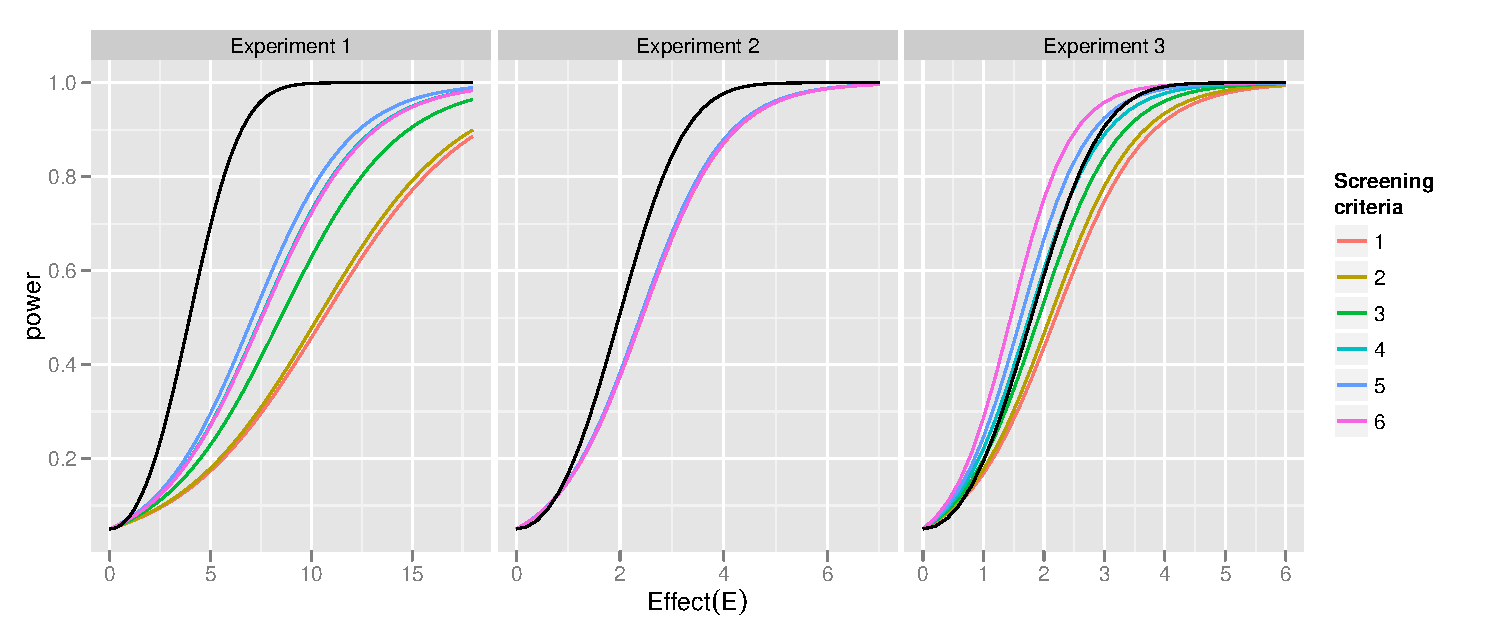
\includegraphics{power_screening.pdf}}
%       \caption{The overall power estimated from mixed model  for each screening criteria are shown. The corresponding power curve for conventional test is shown for comparison.}
%       \label{fig:power_screening}
%\end{figure}

%\begin{figure}[hbtp]
%   \centering
%       \scalebox{0.70}{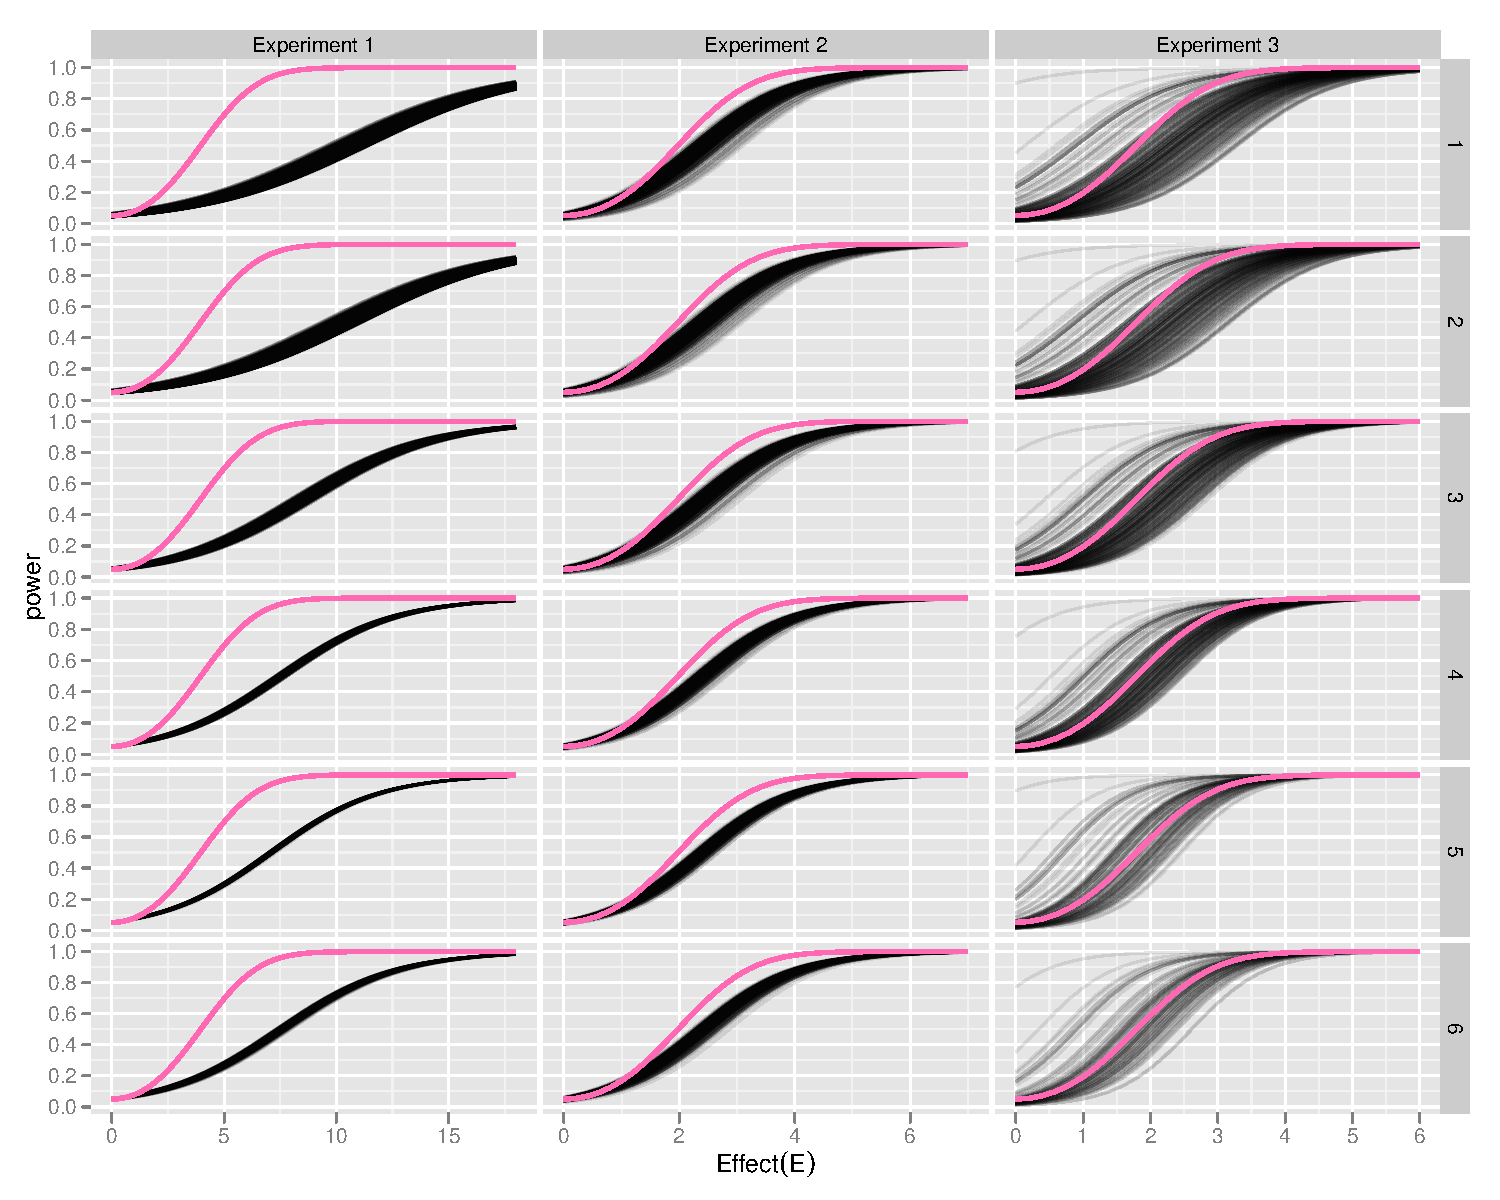
\includegraphics{power_screening_subject.pdf}}
%       \caption{The subject specific power ($K=1$) estimated from mixed model for all the six screening criteria are shown. The corresponding power curves for conventional test is shown for comparison.}
%       \label{fig:power_screening_subject}
%\end{figure}

\begin{table}[hbtp]
\caption{Number of unique subjects and their total feedbacks before and after data cleaning. 
Note that the number of male and female participants may not add up to the number of subjects, due to some participants declining to provide demographic information. }
\begin{center}
\begin{tabular}{rrrrr|rrrr|rrrr}
  \hline
Data &  \multicolumn{4}{c} {Experiment 1}  & \multicolumn{4}{c} {Experiment 2}  & \multicolumn{4}{c} {Experiment 3} \\
 \cline{2-5}  \cline{6-9}   \cline{10-13}
cleaning & Subj & Male & Fem & Total & Subj & Male & Fem & Total & Subj & Male & Fem & Total \\ 
  \hline
before & 424 & 226 & 180 & 4516 & 386 & 199 & 182 & 4330 & 242 & 158 &  79 & 2565 \\ 
after  & 239 & 121 & 107 & 2249 & 351 & 185 & 164 & 3636 & 155 & 103 &  52 & 1511 \\ 
   \hline
\end{tabular}
\end{center}
\label{tbl:summary}
\end{table}

After cleaning the data, for experiment 1, we did not have 300 subjects that we planned for. It was decided that more data was not needed, though, because the estimated with margin of error  with the 239 subjects was close to 0.05. This can be seen from the bootstrap confidence band in Figure \ref{p-fig:power_loess_effect} of the manuscript. With experiments 2 and 3 there was sufficient data even after cleaning. Part of the success with the later experiments comes from the researchers developing a reputation on Amazon for providing a good task and reliable payment, which means the reliable turkers look specifically for these tasks.


\section{How much do null plots affect the choice?} \label{sec:null_choice}

It is discussed in the Section \ref{p-sec:null_choice} of the manuscript that $p$-values can be used to quantify the similarity of the visual pattern in the plots used for the simulation experiments. Based on this, we explore more details on how much the null plots affect the choice made by the subjects. 

We have seen that the subjects tend to pick the plot in the lineup that has the lowest $p$-value (Figure \ref{p-fig:P-val_log2} in the mauscript). What we are also interested in  is how this pick is affected by the distribution  of $p$-values of other plots in the lineup, particularly the $p$-value of the null plot with the strongest structure. If there is a null plot with a small $p$-value, or one close to that of the actual data plot, we would expect that subjects have a harder time detecting the actual data plot. Figure \ref{fig:pval_difference} investigates this. The difference between the $p$-value of the actual data is compared with the lowest from the null plots. This is plotted horizontally, and the proportion correct is plotted vertically. Negative values indicate lineups where the actual data plot had a smaller $p$-value than the minimum of the null plots. In experiment 1 (boxplots) there were a lot of lineups where the actual data plot had the smallest $p$-value, but only just. This caused quite some confusion for subjects, as seen because the variability in the proportion correct is huge for these lineups. Similarly large variability in correctness can be seen in the results of experiment 2 (scatterplots) except that the greater range of of differences in $p$-values shows the strength of subject's ability to pick the plot with most structure. Figure \ref{p-fig:P-val_log2} in the manuscript shed some more light on this story: when there is a big difference between the $p$-values (eg experiment 1, $\beta>7$) the subjects as one force chose the same plot. When there is less difference the distribution of counts is much more evenly spread between plots (eg experiment 1, $\beta=1$). 

In practice, the $p$-value is not going to be a valid way to compare plots. Rather metrics that can measure how graphical elements from one plot to another are perceived similarly are needed. This is investigated in Roy Chowdhury (2012). Here, numerical measures of the similarity between plots are proposed to provide quality metrics for lineups.


\begin{figure}[hbtp]
   \centering
       \scalebox{0.60}{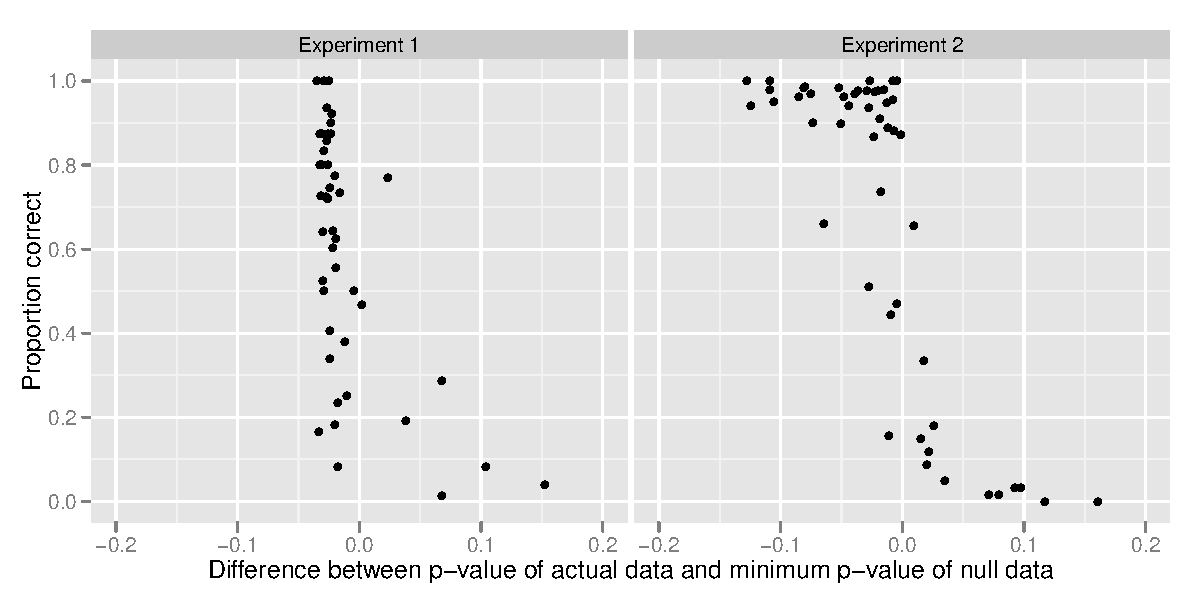
\includegraphics{pval_difference.pdf}}
       \caption{Scatter plot of difference between the data plot's $p$-value and the  smallest $p$-value of the null plots vs proportion correct. Negative differences indicate the $p$-value of the actual data plot are smaller than those of all of the null plots. Difference close to zero shows a wide range in the proportion correct, suggesting that when at least one null plot has structure almost as strong as the actual data plot, subjects had a difficult time in making their choice.}
       \label{fig:pval_difference}
\end{figure}

\section{Type III error}~\label{sec:TypeIII}\label{sec:typeIII_error}


%A little known error amongst statisticians is what was coined as Type III error in \citet{mosteller:48}. This occurs when the null hypothesis is correctly rejected but for the wrong reason. Experiment 3 is prone to this type of error. Observers were asked to identify the plot that had the largest slope, either positive or negative. But the actual data plot had a cluster of points, the contamination that forced the conventional test to fail to see any trend. For the human eye this cluster of points is  as visible as the association between the remaining points, leading the observer to detect the actual data plot by looking for the cluster instead of the slope. This would be considered to be a Type III error because it is not what was requested, but  still gives the correct answer. This is not a problem with the lineup protocol, because we want observers to react to anything that sets the the actual data plot apart. Here, in the controlled but simple setting, it is of interest to see what observers cued to in the actual data plot. 


Figure \ref{p-fig:power_loess_effect} in the manuscript indicates that Type III error might be occurring in experiment 3: correct identification of the actual data plot is not positively associated with effect size. Teasing this out of the results is possible by looking at the reasons participants gave for their choices. Participants were provided with four possible reasons to use for their choice:


\begin{enumerate} \itemsep 0in
\item Most different plot
\item Visible trend
\item Clustering visible
\item Other
\end{enumerate}


\noindent with the possibility to use more than one. The task requested subjects to identify the plot that had the largest slope, which would correspond to choosing ``visible trend'' (2) as the reason for their choice. Reasons 1 or 3 would be indicative of Type III error. Figure \ref{fig:choice_reason} explores the reasons subjects gave for their choices. If there were no Type III errors committed, we would expect that people overwhelmingly using ``visible trend'' as their reason, or at least, when they use this reason they overwhelmingly correctly choose the actual data plot. This is not what we see. At left, are the reasons subjects gave for their choices --- 123 means that they gave all three reasons. The horizontal axis shows proportion of times that subjects correctly chose the actual data plot, and the reasons are sorted from most accurate to least accurate. The size of the point corresponds to the number of subjects putting this as the reason. Subjects that chose all three reasons almost always chose the actual data plot. This was followed by using 1 and 3, and then 1 and 4. The most common reasons given were reasons 1-3 individually, and the accuracy for these reasons ranged from 75\% for reason ``most different plot'' to 60\% for ``visible trend''.
At right is a simplified view, containing just the four possible reasons -- if the subject chose one of these, regardless if they also chose another reason it is counted. ``Visible trend'' comes in third. This is strong evidence that for many subjects even though they are correctly choosing the data plot, often they are cueing to other structure in the plot than the trend, making a Type III error. 

\begin{figure}[hbtp]
   \centering
       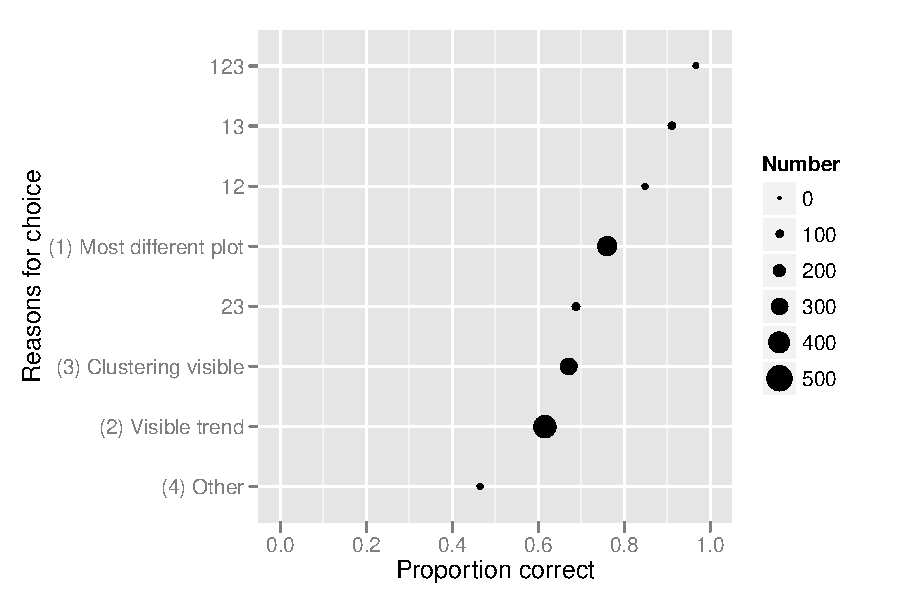
\includegraphics[width=0.45\textwidth]{choice_reason2.pdf}
       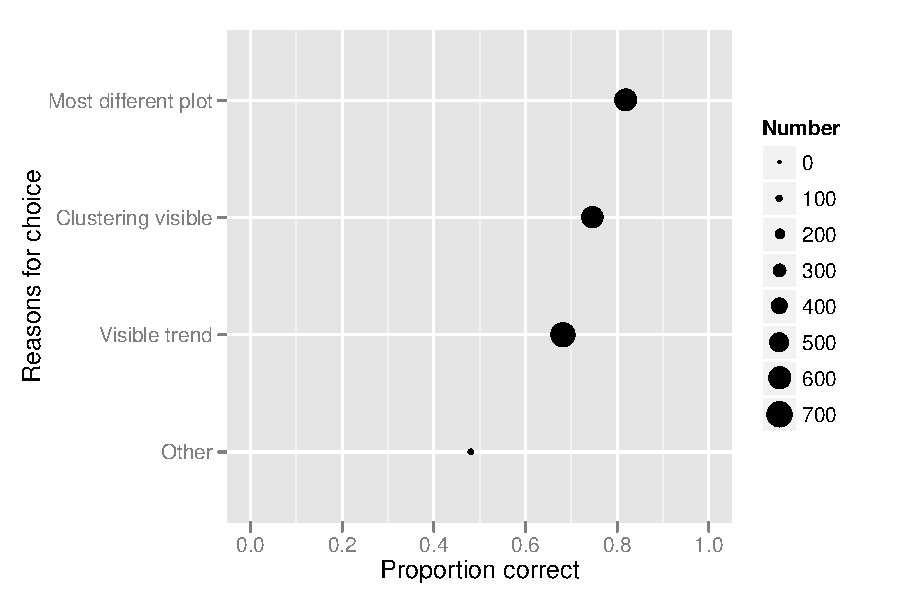
\includegraphics[width=0.45\textwidth]{choice_reason3.pdf}
       \caption{Reasons of plot choices vs  proportion of times the subjects correctly chose the actual data plot for experiment 3 that examines the occurrence of Type III error. At left, all subjects' choices are shown, and reason 123 means all three reasons are used. At right, if the subject used a reason, regardless if they also used more than this reason, they are counted. Size of the point corresponds to the number of subjects using that reason.}
       \label{fig:choice_reason}
\end{figure}

%For visual inference, making a Type III, is not actually a problem. It is only a possibility in this experiment because we are working with known structure. In the real setting, we are excited to see observers detecting the actual data plot, and curious about how they detect it, with all possible reasons encapsulated in the alternative hypothesis. This does show the importance of the qualitative answers that observers give for their choices.




%\bibliographystyle{asa}
%\bibliography{references}

\end{document}
